\documentclass[]{beamer}

\usetheme{CambridgeUS}
%\usecolortheme{dolphin}

\usepackage[english]{babel}    
\usepackage[utf8]{inputenc}
\usepackage{graphicx}
\usepackage{caption}
\usepackage{subfig}
\usepackage{type1ec}
\usepackage[T1]{fontenc}
\usepackage{bbm}
\usepackage{mathtools}
\usepackage{amssymb}
\usepackage{amsmath}
\usepackage{amsthm}
\usepackage{amsfonts} 
\usepackage{pifont}
\usepackage{url}
\usepackage{multirow}
\usepackage{multicol}
\usepackage{fancybox}
\usepackage{colortbl}
\usepackage{soul}
\usepackage{color}
\usepackage{tikz}
\usetikzlibrary{decorations.pathreplacing}
\usepackage{tkz-berge}
\usepackage{rotating}
\usepackage{pdflscape}
\usepackage{afterpage}
\usepackage{capt-of}
\usepackage{comment}
\usepackage{etoolbox}
\usepackage{environ}
\usepackage{dirtytalk}
\usepackage{calc}
\usepackage[style=authortitle,backend=bibtex]{biblatex}
\addbibresource{refs.bib}


\usepackage{algorithm}
\usepackage{algorithmic}

\let\textmdorig\textmd
\let\textscorig\textsc
\let\textttorig\texttt

\usepackage{lmodern}
\usepackage[T1]{fontenc}

\renewcommand<>{\textsc}[1]{%
  \only#2{\textscorig{#1}}%
}



\usetikzlibrary{decorations,arrows,shapes}

\usepackage{complexity}

\newtheoremstyle{named}{}{}{\itshape}{}{\bfseries}{}{.2em}{\thmnote{#3} #1}
\theoremstyle{named}
\newtheorem{class_definition*}{}

\theoremstyle{definition}
%\newtheorem{definition}{Definition}

\theoremstyle{plain}
%\newtheorem{lemma}{Lemma}
%\newtheorem{theorem}{Theorem}
\newtheorem*{theorem*}{Theorem}
%\newtheorem*{corollary}{Corollary}
\newtheorem{observation}{Observation}
\newtheorem*{observation*}{Observation}
\newtheorem{conjecture}{Conjecture}
\newtheorem*{conjecture*}{Conjecture}

\newcommand{\mc}[1]{\mathcal{#1}}

\newcommand{\hypergraph}{\mathcal{H}}

\newcommand{\rank}{\text{rank}}


\newcommand{\biq}{\mathcal{B}}
\newcommand{\clq}{\mathcal{C}}
\newcommand{\str}{\mathcal{S}}
\newcommand{\trans}[1]{\mathbb{T}_{#1}}
\newcommand{\transs}[1]{\mathbb{T}^*_{#1}}
\newcommand{\oblq}[1]{\mathbb{O}_{#1}}

\newcommand{\Hyper}[1]{\hypergraph_{\mc{#1}}}
\newcommand{\Oblq}[1]{\oblq_{\mc{#1}}}
\newcommand{\Trans}[1]{\trans_{\mc{#1}}}

\newcommand{\bigO}[1]{\mathcal{O}\left(#1\right)}
\newcommand{\bigOs}[1]{\mathcal{O}^*\left(#1\right)}

\newcommand{\tsc}[1]{\textsc{#1}}
%\newcommand{\padd}[2]{\pgfmathadd{#1}{#2}}

%\newcommand{\problem}[3]{\medskip\tsc{#1}\par\textit{Instance}: #2\par\textit{Question}: #3\medskip}
\newcommand{\pproblem}[4]{\medskip\tsc{#1}\par\textit{Instance}: #2\par\textit{Parameter}: #3\par\textit{Question}: #4\medskip}

%tikz stuff
\newcommand{\inners}{1.6pt}
\newcommand{\outers}{1pt}

\newcommand{\tdef}[1]{\textit{\textbf{#1}}}

%complexity
\newcommand{\SiP}[1]{\Sigma^{\P}_{#1}}
\newclass{\Hard}{Hard}
\newclass{\Hness}{Hardness}
\newcommand{\NPH}{\NP\text{-}\Hard}
\newclass{\Complete}{Complete}
\newclass{\Ctude}{Complete}
\newclass{\Cness}{Completeness}
\newcommand{\NPc}{\NP\text{-}\Complete}
\newcommand{\NPct}{\NP\text{-}\Ctude}
\newcommand{\NPcness}{\NP\text{-}\Cness}
\newfunc{\dist}{dist}
\newfunc{\girth}{girth}
\newfunc{\nd}{nd}
\newfunc{\YES}{YES}
\newfunc{\NOi}{NO}
\newfunc{\projax}{Proj}
\newfunc{\liftax}{Lift}
\newfunc{\ff}{ff}
\newfunc{\cf}{cf}
\newfunc{\tw}{tw}
\newfunc{\dc}{dc}
\newfunc{\dcc}{d\overline{c}}
\newcommand{\pname}[1]{\textsc{#1}}

\newcommand{\Proj}[1]{\projax_{#1}}
\newcommand{\Lift}[1]{\liftax_{#1}}

\renewcommand{\K}[1]{K_{\mathcal{#1}}}

\renewcommand{\algorithmicrequire}{\textbf{Input:}}
\renewcommand{\algorithmicensure}{\textbf{Output:}}


\newcommand{\CN}[1]{\chi_{\mathcal{#1}}}

\newtoggle{proof_toggle}
\toggletrue{proof_toggle}
%\togglefalse{proof_toggle}

\NewEnviron{tproof} {
    \iftoggle{proof_toggle} {%
        \begin{proof}\BODY\end{proof}}
    {%
    }
}

\newcommand{\ceil}[1]{\left\lceil#1\right\rceil}
\newcommand{\floor}[1]{\left\lfloor#1\right\rfloor}


\makeatletter
\let\@@magyar@captionfix\relax
\setbeamertemplate{footline}
{
  \leavevmode%
  \hbox{%
  \begin{beamercolorbox}[wd=.333333\paperwidth,ht=2.25ex,dp=1ex,center]{author in head/foot}%
    \usebeamerfont{author in head/foot}IPEC 2019~~\beamer@ifempty{\insertshortinstitute}{}{}
  \end{beamercolorbox}%
  \begin{beamercolorbox}[wd=.333333\paperwidth,ht=2.25ex,dp=1ex,center]{title in head/foot}%
    \usebeamerfont{title in head/foot} Finding cuts of bounded degree
  \end{beamercolorbox}%
  \begin{beamercolorbox}[wd=.333333\paperwidth,ht=2.25ex,dp=1ex,right]{date in head/foot}%
    \usebeamerfont{date in head/foot}\insertshortdate{}\hspace*{2em}
    \insertframenumber{} / \inserttotalframenumber\hspace*{2ex} 
  \end{beamercolorbox}}%
  \vskip0pt%
}
\makeatother


\AtBeginSection[]{
  \begin{frame}
  \vfill
  \centering
  \begin{beamercolorbox}[sep=8pt,center,shadow=true,rounded=true]{title}
    \usebeamerfont{title}\insertsectionhead\par%
  \end{beamercolorbox}
  \vfill
  \end{frame}
}


\title{Finding cuts of bounded degree: complexity, FPT and exact algorithms, and kernelization}
\author{\underline{Guilherme C. M. Gomes} \\
        \vspace{10pt}
        {\footnotesize Universidade Federal de Minas Gerais} \\
        \vspace{20pt}
        Ignasi Sau \\
        \vspace{10pt}
        {\footnotesize CNRS/LIRMM}}
\date{}


\begin{document}
\begin{frame}
	\titlepage
\end{frame}

\subsection{Matching Cut}
\begin{frame}{\pname{Matching Cut}}
    \begin{block}{}
        A matching cut is a bipartition of $V(G)$ such that each vertex has at most one neighbor in the other part.
    \end{block}
    \pause
    
    \begin{figure}[!htb]
        \centering
        \hspace{-0.5cm}
        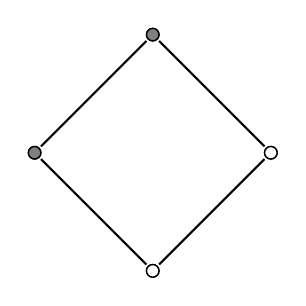
\begin{tikzpicture}[scale=1]
                %\draw[help lines] (-5,-5) grid (5,5);
                \GraphInit[unit=3,vstyle=Simple]
                \SetVertexSimple[Shape=circle, FillColor=black, MinSize=2pt]
                \tikzset{VertexStyle/.append style = {inner sep = \inners, outer sep = \outers}}
                \SetVertexNoLabel
                \grCycle[RA=1.5, prefix=c]{4}
                \AddVertexColor{white}{c0,c3}
                \AddVertexColor{black!50}{c1,c2}
        \end{tikzpicture}
        \pause
        \hspace{1.5cm}
        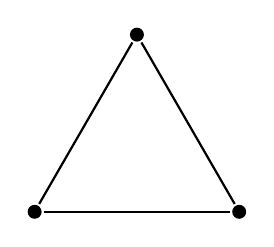
\begin{tikzpicture}[scale=1,rotate=90]
                %\draw[help lines] (-5,-5) grid (5,5);
                \GraphInit[unit=3,vstyle=Simple]
                \SetVertexSimple[Shape=circle, FillColor=black, MinSize=2pt]
                \tikzset{VertexStyle/.append style = {inner sep = \inners, outer sep = \outers}}
                \SetVertexNoLabel
                \grCycle[RA=1.5, prefix=t]{3}
        \end{tikzpicture}
        \pause
        \hspace{1.75cm}
        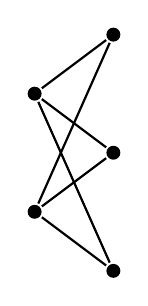
\begin{tikzpicture}[scale=1, rotate=-90, shift={(0,0)}]
                %\draw[help lines] (-5,-5) grid (5,5);
                \GraphInit[unit=3,vstyle=Simple]
                \SetVertexSimple[Shape=circle, FillColor=black, MinSize=2pt]
                \tikzset{VertexStyle/.append style = {inner sep = \inners, outer sep = \outers}}
                \SetVertexNoLabel
                \grCompleteBipartite[RA=1.5, RB = 1.5, RS=1]{2}{3}
        \end{tikzpicture}
    \end{figure}
    \pause
    \fullcite{matching_cut_graham}
    \begin{block}{}
        Which graphs admit a matching cut?
    \end{block}
\end{frame}

\begin{frame}{\pname{Matching Cut} and graph classes}
    \fullcite{chvatal_matching_cut}
    \pause
    \begin{block}{}
        Recognizing these graphs is $\NPH$ even if $\Delta(G) = 4$...
    \end{block}
    \pause
    \fullcite{matching_cut_planar}
    \begin{block}{}
        ...$G$ is planar...
    \end{block}
    \pause
    \fullcite{stable_cutset_line_graphs}
    \begin{block}{}
        ...or $G$ is bipartite.
    \end{block}
\end{frame}

\begin{frame}{Algorithmic results for \pname{Matching Cut}}
    \fullcite{marx_treewidth_reduction}
    \begin{block}{}
        $\FPT$ parameterized by the number of edges crossing the cut.
    \end{block}
    \pause
    \fullcite{matching_cut_tcs}
    \begin{block}{}
        $\FPT$ parameterized by vertex cover; $\bigOs{2^{n/2}}$ exact exponential algorithm.
    \end{block}
\end{frame}

\begin{frame}{Algorithmic results for \pname{Matching Cut}}
    \fullcite{matching_cut_structural}
    \begin{block}{}
        $\FPT$ parameterized by treewidth, neighborhood diversity, or twin cover.
    \end{block}
\end{frame}


\begin{frame}{Algorithmic results for \pname{Matching Cut}}
    \fullcite{matching_cut_ipec}
    \begin{block}{}
        \begin{itemize}
            \item $\FPT$ parameterized by distance to cluster, distance to co-cluster;
            \item Quadratic kernel for distance to cluster, linear kernel for distance to clique;
            \item No polynomial kernel for treewidth $+$ number of crossing edges $+$ maximum degree (unless $\NP \subseteq \coNP/\poly$).
            \item Exact exponential running in $\bigOs{1.38^n}$.
        \end{itemize}
    \end{block}
    \pause
    \begin{block}{}
        During their presentation, asked for results on the generalization of \pname{Matching Cut} we discuss here.
    \end{block}
\end{frame}

\begin{frame}{Cuts and degree constraints}
    %\setbeamercovered{transparent}
    \onslide<1-4>
    \begin{block}{}
        A matching cut is a bipartition of $V(G)$ such that each vertex has at most one neighbor in the other part.
    \end{block}
    \onslide<2-5>
    \begin{block}{Option 1}
        Look for a \textbf{bipartition} such that each vertex has at most $\boldsymbol{d}$ neighbors in the other part.
    \end{block}
    \onslide<3-4>
    \begin{block}{Option 2}
        Look for a \textbf{$\boldsymbol{p}$-partition} such that each vertex has at most \textbf{one} neighbor outside its part.
    \end{block}
    \onslide<4-4>
    \begin{block}{Option 3}
        Look for a \textbf{$\boldsymbol{p}$-partition}  such that each pair of parts forms a matching cut.
    \end{block}
    %\setbeamercovered{invisible}
\end{frame}

\begin{frame}{Some definitions}
    \begin{block}{}
        A bipartition $(A,B)$ of $V(G)$ is a $d$-cut if and only if each vertex has at most $d$ neighbors across the cut.
    \end{block}
    
    
    \begin{figure}[!htb]
        \centering
        \onslide<2->
        \hspace{-0.4cm}
        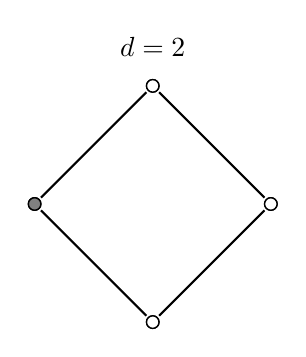
\begin{tikzpicture}[scale=1]
                %\draw[help lines] (-5,-5) grid (5,5);
                \node at (0,2) {$d=2$};
                \GraphInit[unit=3,vstyle=Simple]
                \SetVertexSimple[Shape=circle, FillColor=black, MinSize=2pt]
                \tikzset{VertexStyle/.append style = {inner sep = \inners, outer sep = \outers}}
                \SetVertexNoLabel
                \grCycle[RA=1.5, prefix=c]{4}
                \AddVertexColor{white}{c0,c1,c3}
                \AddVertexColor{black!50}{c2}
        \end{tikzpicture}
        \onslide<3->
        \hspace{1.4cm}
        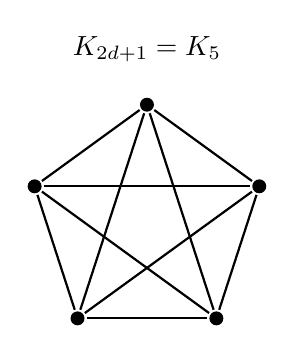
\begin{tikzpicture}[scale=1,rotate=90]
                %\draw[help lines] (-5,-5) grid (5,5);
                \GraphInit[unit=3,vstyle=Simple]
                \SetVertexSimple[Shape=circle, FillColor=black, MinSize=2pt]
                \onslide<6->{\node at (2.2,0) {$K_{2d+1} = K_5$};}
                \tikzset{VertexStyle/.append style = {inner sep = \inners, outer sep = \outers}}
                \SetVertexNoLabel
                \grComplete[RA=1.5,prefix=p]{5}
        \end{tikzpicture}
        \onslide<4->
        \hspace{1cm}
        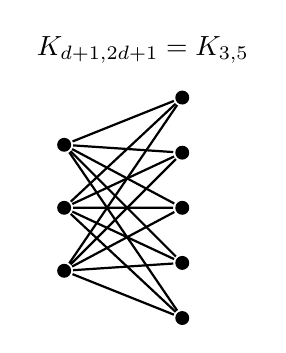
\begin{tikzpicture}[scale=1, rotate=-90]
                %\draw[help lines] (-5,-5) grid (5,5);
                \GraphInit[unit=3,vstyle=Simple]
                \SetVertexSimple[Shape=circle, FillColor=black, MinSize=2pt]
                \tikzset{VertexStyle/.append style = {inner sep = \inners, outer sep = \outers}}
                \SetVertexNoLabel
                \onslide<7->{\node at (-0.6,1) {$K_{d+1,2d+1} = K_{3,5}$};}
                \grCompleteBipartite[RA=0.8, RB = 0.7, RS=1.5]{3}{5}
        \end{tikzpicture}
    \end{figure}
    \onslide<5->
    \begin{block}{}
        A set $S \subseteq V(G)$ is \textit{monochromatic} if, in every $d$-cut $(A, B)$, it holds that $S \subseteq A$ or $S \subseteq B$.
    \end{block}
\end{frame}

\begin{frame}{Regular graphs are hard}
    \begin{theorem}
        \pname{$d$-Cut} on $(2d+2)$-regular graphs is $\NPH$.
    \end{theorem}
    \pause
    \begin{block}{\pname{3-Uniform Hypergraph Bicoloring}}
        \textit{Instance}: A hypergraph $\mathcal{H}$ with three vertices in each hyperedge.
        \textit{Question}: Can we 2-color $V(\mathcal{H})$ such that no hyperedge is monochromatic?
    \end{block}
    \pause
    \begin{block}{}
        Heavily inspired on the reduction given by:  \fullcite{chvatal_matching_cut}.
    \end{block}
\end{frame}

\begin{frame}{Monochromatic gadget: Spools}
    \begin{columns}[T]
        \begin{column}{0.44\textwidth}
        \begin{figure}[!htb]
            \centering
            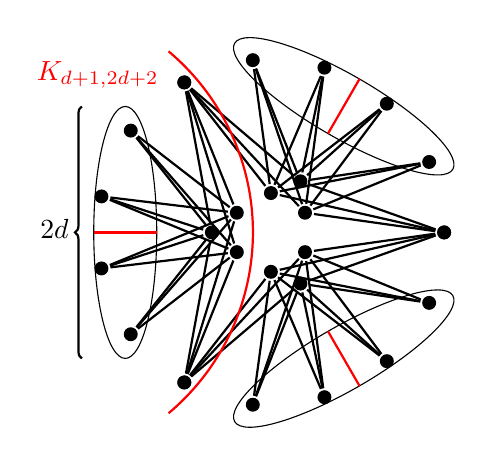
\begin{tikzpicture}[scale=1]
                %\draw[help lines] (-5,-5) grid (5,5);
                \GraphInit[unit=3,vstyle=Simple]
                \SetVertexSimple[Shape=circle, FillColor=black, MinSize=1pt]
                \tikzset{VertexStyle/.append style = {inner sep = \inners, outer sep = \outers}}
                \SetVertexNoLabel
                \foreach \x in {0,1,2} {
                    \pgfmathtruncatemacro{\med}{(\x)*120 + 30}
                    \begin{scope}[rotate=-\med]
                        \draw (0,1.85) ellipse (1.6cm and 0.4cm);
                        \onslide<6>{\draw[thick, color=red] (0,1.45) -- (0,2.25);}
                    \end{scope}
                    \foreach \y in {0,1,2,3,4,5} {
                        \pgfmathtruncatemacro{\ang}{\x * 120 + \y * 24}
                        \Vertex[a=\ang, d=2.2]{i\x\y}
                    }
                    \foreach \y in {0,1,2} {
                        \pgfmathtruncatemacro{\ang}{\x * 120 + \y * 30 + 30}
                        \pgfmathsetmacro{\bla}{0.5 + mod(\y,2) *0.25}
                        \Vertex[a=\ang, d=\bla]{o\x\y}
                        \foreach \z in {0,1,2,3,4,5} {
                            \Edge(i\x\z)(o\x\y)
                        }
                    }
                }
                \onslide<2>{
                    \draw[thick,color=red] (-1.3,2.3) arc (50:-50:3);
                    \node[color=red] at (-2.2, 2) {$K_{d+1, 2d+2}$};
                }
                
                \onslide<3->{
                    \draw[decorate, decoration={brace, mirror}, thick] (-2.4,1.6) --(-2.4,-1.6);
                    \node at (-2.75, 0.05) {$2d$};
                }
            \end{tikzpicture}
        \end{figure}
        \end{column}
        \hfill
        \begin{column}{0.5\textwidth}
            \begin{itemize}
                \onslide<4->
                \item Create one spool for each vertex $v$ and one for each color. \textbf{Goal}: if there is no bicoloring of the hypergraph,
                      the whole graph is monochromatic.
                \onslide<5->
                \item Assign an unique label to each set of circled vertices.
                \onslide<6->
                \item Divide each of them in two equal sized sets. Add edges within and between these sets to encode the hyperedges and achieve regularity.
            \end{itemize}
        \end{column}
    \end{columns}
\end{frame}

\begin{frame}{Why regularity is important}
    \begin{block}{}
        There is a very similar problem known as \pname{Internal Partitions}, where we want a bipartition of $V(G)$ such that every vertex has at least half of its neighbors on its own part.
    \end{block}
    \pause
    \fullcite{internal_partition_regular6}
    \begin{conjecture}
        For every $r$, there is a constant $n_r$ such that every $r$-regular graph with at least $n_r$ vertices has an internal partition (open since 2002). Known to hold for $r=3,4,6$.
    \end{conjecture}
    \pause
    \begin{block}{}
        Improving upon our reduction would imply that the conjecture is false (or $\P = \NP$), while polynomial algorithms would likely yield a proof.
    \end{block}{}
\end{frame}

\begin{frame}{Some polynomial cases}
    \fullcite{chvatal_matching_cut}
    \begin{block}{}
        \pname{Matching Cut} can be solved in polynomial time for graphs of maximum degree at most 3.
    \end{block}
    \pause
    \begin{theorem}
        If $\Delta(G) \leq d+2$, \pname{$d$-Cut} can be solved in polynomial time.
    \end{theorem}
    \pause
    \begin{block}{}
        \textit{Sketch of the proof}: find a shortest cycle $C$.
        If there is some vertex with too many neighbors in $C$, we either find a shorter cycle, or we have that $d = 2$ and extend $C$ to $Q$ until $(Q, G - Q)$ is a $d$-cut or $G$ is monochromatic.
    \end{block}
\end{frame}

\section{Parameterized algorithms}

\begin{frame}{Kernelization}
    \begin{theorem}
        \pname{$d$-Cut} does not admit a polynomial kernel when parameterized by treewidth, number of crossing edges and maximum degree, unless $\NP \subseteq \coNP/\poly$.
    \end{theorem}
    \onslide<2->
    \begin{block}{}
        We show that \pname{$d$-Cut} (OR-)cross-composes onto itself.
    \end{block}
    \onslide<3->
    \begin{figure}[!htb]
        \centering
        \hspace{-0.5cm}
        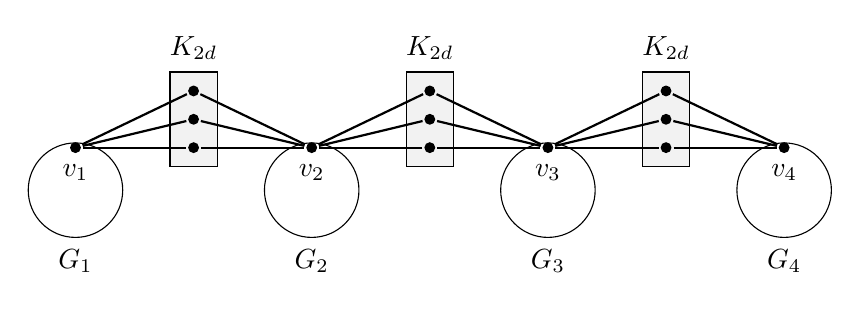
\begin{tikzpicture}[scale=0.6]
            \GraphInit[unit=3,vstyle=Normal]
            \SetVertexNormal[Shape=circle, FillColor=black, MinSize=1pt]
            \tikzset{VertexStyle/.append style = {inner sep = 1.2, outer sep = \outers}}
            \onslide<4->
            \foreach \i in {0,1,2,3} {
                \pgfmathsetmacro{\x}{5*\i}
                \pgfmathtruncatemacro{\id}{\i + 1}
                \draw (\x,0) circle (1);
                \node at (\x, -1.5) {$G_\id$};
            }
            \onslide<5->
            \foreach \i in {0,1,2,3} {
                \pgfmathsetmacro{\x}{5*\i}
                \pgfmathtruncatemacro{\id}{\i + 1}
                \Vertex[x=\x, y=0.9, LabelOut, Lpos=270, L={v_\id}, Math]{v_\i}
            }
            \onslide<6->
            \foreach \i in {0,1,2} {
                \pgfmathsetmacro{\x}{5*\i + 2}
                \pgfmathsetmacro{\xp}{\x+1}
                \pgfmathsetmacro{\xk}{\x+0.5}
                \pgfmathtruncatemacro{\id}{\i + 1}
                \draw[fill=gray!10] (\x, 0.5) rectangle (\xp, 2.5);
                \node at (\xk, 3) {$K_{2d}$};
                \Vertex[x=\xk, y=2.1, NoLabel]{x_0\i}
                \Vertex[x=\xk, y=1.5, NoLabel]{x_1\i}
                \Vertex[x=\xk, y=0.9, NoLabel]{x_2\i}
                \foreach \j in {0,1,2} {
                    \Edge(x_\j\i)(v_\i)
                    \Edge(x_\j\i)(v_\id)
                }
            }
        \end{tikzpicture}
    \end{figure}
\end{frame}

\begin{frame}{Distance to (co-)cluster}
    \begin{block}{}
        $G$ is a cluster graph if each of its connected components is a clique (cluster).
    \end{block}
    \onslide<2->
    \begin{figure}[!htb]
        \centering
        \hspace{-0.5cm}
        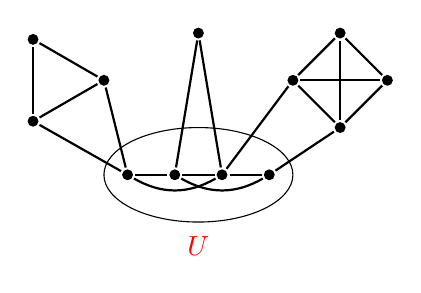
\begin{tikzpicture}[scale=0.6]
            \GraphInit[unit=3,vstyle=Normal]
            \SetVertexNormal[Shape=circle, FillColor=black, MinSize=1pt]
            \tikzset{VertexStyle/.append style = {inner sep = 1.2, outer sep = \outers}}
            \SetVertexNoLabel
            \begin{scope}[shift={(-3, 2)}]
                \grComplete[RA=1,prefix=t]{3}
            \end{scope}
            
            \begin{scope}[shift={(3, 2)}]
                \grComplete[RA=1,prefix=s]{4}
            \end{scope}
            
            \begin{scope}[shift={(-1, 3)}]
                \grComplete[RA=1,prefix=v]{1}
            \end{scope}
            
            \onslide<2-3>{
                \begin{scope}[shift={(-1.5, 0)}]
                    \grPath[RA=1, prefix=p]{4}
                    \Edge[style=bend right](p0)(p2)
                    \Edge[style=bend right](p1)(p3)
                \end{scope}
                \Edge(v0)(p1)
                \Edge(v0)(p2)
                
                \Edge(s2)(p2)
                \Edge(s3)(p3)
                
                \Edge(t0)(p0)
                \Edge(t2)(p0)
                
                
                \onslide<3> {
                    \draw (0,0) ellipse (2cm and 1cm);
                    \node[color=red] at (0, -1.5) {$U$};
                }
            }
        \end{tikzpicture}
    \end{figure}
    \onslide<3->
    \begin{block}{}
        The modulator $U \subset V(G)$ is a set such that $G - U$ is a cluster graph, with clusters $\{C_1, \dots, C_{\ell}\}$.
    \end{block}
    \onslide<5>
    \begin{block}{}
        A co-cluster graph is the complement graph of a cluster graph.
    \end{block}
\end{frame}


\begin{frame}{The basics}
    \begin{block}{Key idea}
        Partition $U$ in monochromatic sets $\{U_1, \dots, U_\ell\}$ and merge them until we get a kernel.
    \end{block}
\end{frame}

\begin{frame}{$N^{2d}(U_i)$}
    \vspace{-0.3cm}
    \begin{block}{}
        For each $U_i$, a vertex $v \in V(G) \setminus U$ is in $N^{2d}(U_i)$ if:
        \begin{itemize}
            \item<2->[1] $v$ has at least $d+1$ neighbors in $U_i$; or
            \item<3->[2] $v$ is in a cluster $C$ of size at least $2d+1$ in $G - U$ such that there is some vertex of $C$ with at least $d+1$ neighbors in $U_i$; or
            \item<4->[3] $v$ is in a cluster $C$ and some vertex in $U_i$ has $2d$ neighbors in $C$; or
            \item<5->[4] $v$ is in a cluster $C$ of size at least $2d+1$ and there is some vertex in $U_i$ with $d+1$ neighbors in $C$.
        \end{itemize}
    \end{block}
    \begin{figure}[!htb]
        \centering
        \hspace*{1cm}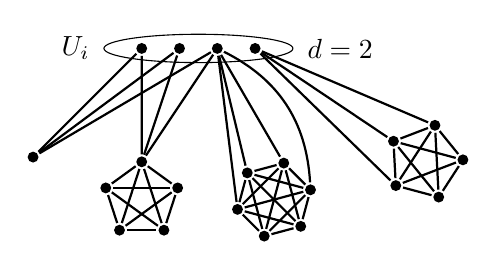
\begin{tikzpicture}[scale=0.6]
            \GraphInit[unit=3,vstyle=Normal]
            \SetVertexNormal[Shape=circle, FillColor=black, MinSize=1pt]
            \tikzset{VertexStyle/.append style = {inner sep = 1.2, outer sep = \outers}}
            \SetVertexNoLabel
            \node at (-2.6, 0) {$U_i$};
            \node at (3, 0) {$d=2$};
            \draw (0,0) ellipse (2cm and 0.3cm);
            \Vertex[x=-1.2, y=0]{x0}
            \Vertex[x=-0.4, y=0]{x1}
            \Vertex[x=0.4, y=0]{x2}
            \Vertex[x=1.2, y=0]{x3}
            
            \onslide<2->{
                \Vertex[x=-3.5, y=-2.3]{c1}
                \Edge(c1)(x0)
                \Edge(c1)(x1)
                \Edge(c1)(x2)
            }
            
            \onslide<3-> {
                \begin{scope}[scale=0.8, shift={(-1.5,-4)}]
                    \tikzset{VertexStyle/.append style = {inner sep = 1.2pt, outer sep = \outers}}
                    \begin{scope}[rotate=90]
                        \grComplete[RA=1, prefix=p]{5}
                    \end{scope}
                    \Edge(p0)(x0)
                    \Edge(p0)(x1)
                    \Edge(p0)(x2)
                \end{scope}
            }
            
            \onslide<4->{
                \begin{scope}[scale=0.8, shift={(2,-4)}]
                    \tikzset{VertexStyle/.append style = {inner sep = 1.2pt, outer sep = \outers}}
                    \begin{scope}[rotate=75]
                        \grComplete[RA=1, prefix=t]{6}
                    \end{scope}
                    \Edge(x2)(t0)
                    \Edge(x2)(t1)
                    \Edge[style = bend left](x2)(t5)
                    \Edge(x2)(t2)
                \end{scope}
                
                \onslide<5->
                \begin{scope}[scale=0.8, shift={(6,-3)}]
                    \tikzset{VertexStyle/.append style = {inner sep = 1.2pt, outer sep = \outers}}
                    \begin{scope}[rotate=75]
                        \grComplete[RA=1, prefix=q]{5}
                    \end{scope}
                    \Edge(x3)(q0)
                    \Edge(x3)(q1)
                    \Edge(x3)(q2)
                \end{scope}
            }
        \end{tikzpicture}
    \end{figure}
\end{frame}

\begin{frame}{The kernel}
    
    \begin{theorem}
        When parameterized by distance to cluster, \pname{$d$-Cut} admits a polynomial kernel with $\bigO{d^2\dc(G)^{2d+1}}$ vertices that can be computed in $\bigO{d^4\dc(G)^{2d+1}(n+m)}$ time.
    \end{theorem}

\end{frame}

\begin{frame}{Number of crossing edges}
    \begin{block}{}
        We can solve \pname{$d$-Cut} in $\FPT$ time using the treewidth reduction technique.
    \end{block}
    \fullcite{marx_treewidth_reduction}
    \pause
    \begin{block}{}
        We cast \pname{$d$-Cut} as a separation problem on the line graph: for some pair $s,t \in V(L(G))$, we want a cutset with a maximum clique of size $\leq d$.
    \end{block}
    \pause
    \begin{theorem}{}
      \textsc{$d$-Cut} is \FPT\ paramterized by the number of crossing edges.
    \end{theorem}
\end{frame}

\begin{frame}{Treewidth}
    \begin{block}{}
        Dynamic programming on a nice tree decomposition.
    \end{block}
    \begin{columns}[T]
        \begin{column}{0.4\textwidth}
            \vspace{-0.5cm}
            \begin{figure}[!htb]
                \centering
                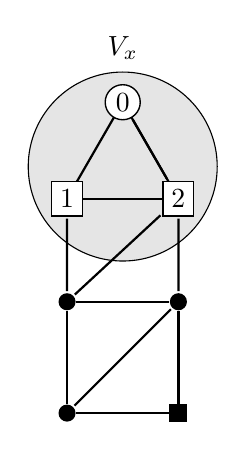
\begin{tikzpicture}[rotate = 0]
                        %\draw[help lines] (-5,-5) grid (5,5);
                        \GraphInit[unit=3,vstyle=Normal]
                        \SetVertexNormal[Shape=circle, MinSize=3pt]
                        \tikzset{VertexStyle/.append style = {inner sep = \inners, outer sep = \outers}}
                        \SetVertexNoLabel
                        \begin{scope}[rotate=90]
                            \draw[fill=gray!20] (0,0) circle (1.2);
                            \node at (1.5, 0) {$V_x$};
                            \grComplete[RA=0.816747, prefix=t]{3}
                            \SetVertexLabel
                            \Vertex[Node, L = {0}, Math]{t0}
                        \end{scope}
                        \begin{scope}[rotate=90]
                            \tikzset{VertexStyle/.append style = {inner sep = 3pt, shape = rectangle}}
                            \SetVertexLabel
                            \Vertex[Node, L = {2}, Math]{t2}
                            \Vertex[Node, L = {1}, Math]{t1}
                        \end{scope}
                        \begin{scope}[rotate=45, shift={(-1.71424, -1.71424)}]
                            \grCycle[RA=1, prefix=c]{4}
                            \Edge(t0)(t2)
                        \end{scope}
                        \begin{scope}[rotate=45, shift={(-1.71424, -1.71424)}]
                            \SetVertexNormal[Shape=circle, FillColor = black, MinSize=3pt]
                            \tikzset{VertexStyle/.append style = {shape = rectangle, inner sep = 3pt, outer sep = \outers}}
                            \Vertex[Node]{c3}
                        \end{scope}
                        \begin{scope}[rotate=45, shift={(-1.71424, -1.71424)}]
                            \SetVertexNormal[Shape=circle, FillColor = black, MinSize=3pt]
                            \tikzset{VertexStyle/.append style = {inner sep = 2pt, outer sep = \outers}}
                            \Vertex[Node]{c0}
                            \Vertex[Node]{c1}
                            \Vertex[Node]{c2}
                        \end{scope}
                        \Edge(c0)(t2)
                        \Edge(c1)(t2)
                        \Edge(c1)(t1)
                        \Edge(c0)(c2)
                        %\AssignVertexLabel{t}{0,1,0}
                \end{tikzpicture}
            \end{figure}
        \end{column}
        \begin{column}{0.55\textwidth}
            \begin{itemize}
                \item<2-> $S \subseteq V_x$ represents which (squared) elements of $V_x$ are assigned to $A$.
                \item<3-> $\mathbf{\alpha} \in \{0, \dots, d\}^{|V_x|}$ stores how many neighbors each $v \in V_x$ has across the cut \textbf{\textit{outside}} of $V_x$.
                \item<4-> $t = 1$ if $A$ and $B$ are non-empty. 
                \item<5-> $f_x(S, \mathbf{\alpha}, t) = 1$ iff the subtree rooted at bag $x$ has a partition that satisfies all of the above.
            \end{itemize}
        \end{column}
    \end{columns}
\end{frame}

\begin{frame}{Treewidth}
    \begin{theorem}
        For every $d \geq 1$, \pname{$d$-Cut} can be solved in $\bigOs{2^{\tw(G)}(d+1)^{2\tw(G)}}$.
    \end{theorem}
    \pause
    \begin{corollary}
        \pname{Matching Cut} can be solved in $\bigOs{8^{\tw(G)}}$. (Improvement upon $12^{\tw(G)}$).
    \end{corollary}
    \fullcite{matching_cut_structural}
\end{frame}

\begin{frame}{Other results}
    \begin{theorem}
        \pname{$d$-Cut} can be solved in $\bigOs{(d+1)^{\dc(G)}}$ time.
    \end{theorem}
    \pause
    \begin{theorem}
        \pname{$d$-Cut} can be solved in $\bigOs{(d+1)^{\dcc(G)}}$ time.
    \end{theorem}
\end{frame}

\begin{frame}{Open Problems}
    \begin{block}{}
        Settle the complexity for graphs of maximum degree between $d+3$ and $2d+1$.
        We guess most of these should be solvable in polynomial time, but right now we have no idea how to tackle this problem.
    \end{block}
    \pause
    \begin{block}{}
        Decide if the exponential dependency on $d$ is necessary, or if we can restrict its influence to a polynomial factor.
    \end{block}
    \pause
    \begin{block}{}
        Explore the other generalizations of \pname{Matching Cut}, in particular Option 3, which seems considerably harder than the other two.
    \end{block}
    \begin{block}{Option 3}
        Look for a \textbf{$\boldsymbol{p}$-partition}  such that each pair of parts forms a matching cut.
    \end{block}
\end{frame}


\section{Thank you!}

\end{document}
